\documentclass{exam}
\usepackage{graphicx}
\usepackage[utf8]{inputenc}
\usepackage[main=english,vietnamese]{babel}
\usepackage{amsmath}
\usepackage{hyperref}
\usepackage{amsthm}
\usepackage{tcolorbox}
\usepackage{amsfonts}
\usepackage{amssymb}
\usepackage{mathrsfs}
\usepackage{centernot}
\usepackage{cases}
\usepackage{physics}
\usepackage[shortlabels]{enumitem}
\usepackage{tikz}
\usepackage{lipsum}
\usepackage{sidecap}
\usepackage{verbatim}
\usepackage{listings}
\usepackage{kvmap}

\usetikzlibrary{calc}
\usetikzlibrary{decorations.pathmorphing}

\definecolor{borderblue}{HTML}{33c2ff}
\definecolor{codegreen}{rgb}{0,0.6,0}
\definecolor{codegray}{rgb}{0.5,0.5,0.5}
\definecolor{codepurple}{rgb}{0.58,0,0.82}
\definecolor{backcolour}{rgb}{0.95,0.95,0.92}

\lstdefinestyle{mystyle}{
    backgroundcolor=\color{backcolour},   
    commentstyle=\color{codegreen},
    keywordstyle=\color{magenta},
    numberstyle=\tiny\color{codegray},
    stringstyle=\color{codepurple},
    basicstyle=\ttfamily\footnotesize,
    breakatwhitespace=false,         
    breaklines=true,                 
    captionpos=b,                    
    keepspaces=true,                 
    numbers=left,                    
    numbersep=5pt,                  
    showspaces=false,                
    showstringspaces=false,
    showtabs=false,
    tabsize=2
}

\lstset{style=mystyle}

\newcommand{\paren}[1]{\left(#1\right)}
\newcommand{\curly}[1]{\left\{#1\right\}}

\allowdisplaybreaks

\makeatletter
\long\def\paragraph{%
  \@startsection{paragraph}{4}%
  {\z@}{2ex \@plus 1ex \@minus .2ex}{-1em}%
  {\normalfont\normalsize\bfseries}%
}
\makeatother

\makeatletter
\def\@xequals@fill{\arrowfill@\Relbar\Relbar\Relbar}
\newcommand*\xequals[2][]{\DOTSB\ext@arrow0055\@xequals@fill{#1}{#2}}
\makeatother

\makeatletter
\renewcommand*\env@matrix[1][*\c@MaxMatrixCols c]{%
  \hskip -\arraycolsep
  \let\@ifnextchar\new@ifnextchar
  \array{#1}}
\makeatother

\NewTColorBox{algorithm}{m}{
  standard jigsaw,
  sharp corners,
  boxrule=0.4pt,
  coltitle=black,
  colframe=black,
  opacityback=0,
  opacitybacktitle=0,
  fonttitle=\normalfont\bfseries\upshape,
  fontupper=\normalfont,
  title={Algorithm #1},
  after title={.},
  attach title to upper={\ },
}

\NewTColorBox{question}{m}{
  standard jigsaw,
  sharp corners,
  boxrule=0.4pt,
  coltitle=black,
  colframe=black,
  opacityback=0,
  opacitybacktitle=0,
  fonttitle=\normalfont\bfseries\upshape,
  fontupper=\normalfont,
  title={Question #1},
  attach title to upper={\ },
}

\newcommand{\lnand}{\uparrow}
\newcommand{\lnor}{\downarrow}

\title{ECE341 - Homework 3}
\author{Ton-Minh-Ky Tran}
\date{\today}

\begin{document}

\maketitle

\section{Cathode 7-segment display implementation using basic logic gates}
\begin{figure}[ht]
	\centering
	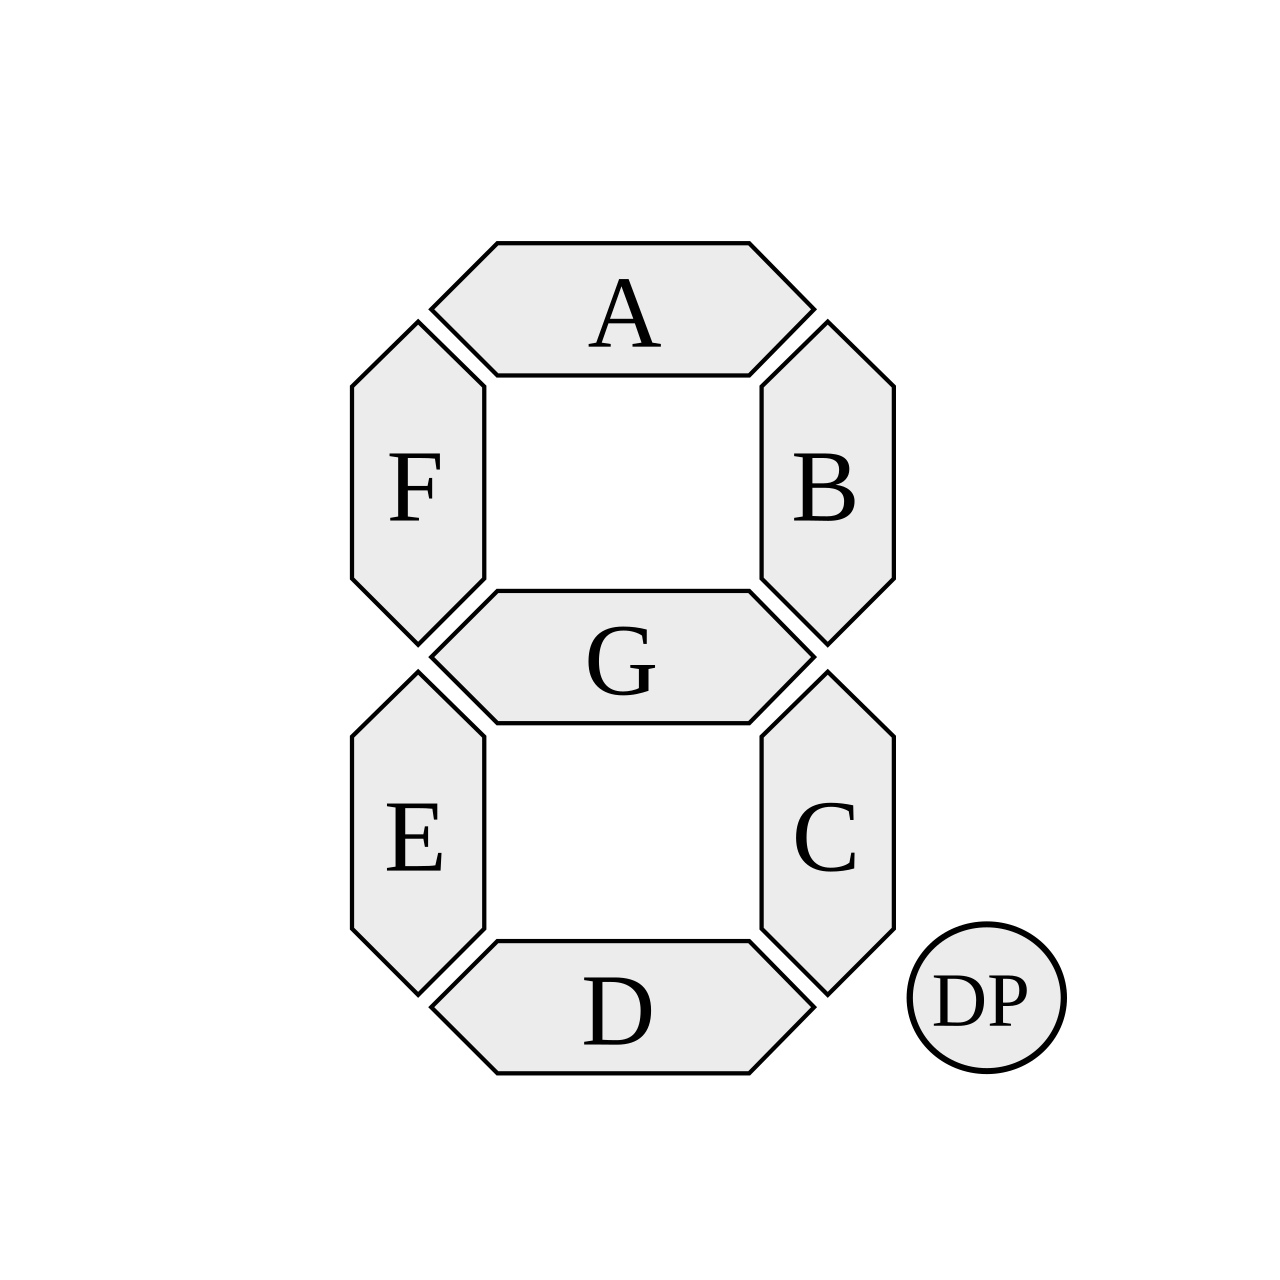
\includegraphics[width=0.2\linewidth]{7sd.png}
	\caption{Seven-segment display}
\end{figure}
Using the above seven-segment display segments naming convention, we devise a truth table for every number determining which segment to enable (decimal point is not used). Denote by $w_3$, $w_2$, $w_1$, $w_0$ the number's most significant bit to the least significant bit; then we have the following:

\begin{center}
	\bgroup
	\def\arraystretch{1.2}
	\begin{tabular}{|cccc|ccccccc|}
		\hline
		$w_3$ & $w_2$ & $w_1$ & $w_0$ & $A$ & $B$ & $C$ & $D$ & $E$ & $F$ & $G$ \\
		\hline
		0 & 0 & 0 & 0 & 1 & 1 & 1 & 1 & 1 & 1 & 0 \\
		0 & 0 & 0 & 1 & 0 & 1 & 1 & 0 & 0 & 0 & 0 \\
		0 & 0 & 1 & 0 & 1 & 1 & 0 & 1 & 1 & 0 & 1 \\
		0 & 0 & 1 & 1 & 1 & 1 & 1 & 1 & 0 & 0 & 1 \\
		0 & 1 & 0 & 0 & 0 & 1 & 1 & 0 & 0 & 1 & 1 \\
		0 & 1 & 0 & 1 & 1 & 0 & 1 & 1 & 0 & 1 & 1 \\
		0 & 1 & 1 & 0 & 1 & 0 & 1 & 1 & 1 & 1 & 1 \\
		0 & 1 & 1 & 1 & 1 & 1 & 1 & 0 & 0 & 0 & 0 \\
		1 & 0 & 0 & 0 & 1 & 1 & 1 & 1 & 1 & 1 & 1 \\
		1 & 0 & 0 & 1 & 1 & 1 & 1 & 1 & 0 & 1 & 1 \\
		1 & 0 & 1 & 0 & 1 & 1 & 1 & 0 & 1 & 1 & 1 \\
		1 & 0 & 1 & 1 & 0 & 0 & 1 & 1 & 1 & 1 & 1 \\
		1 & 1 & 0 & 0 & 1 & 0 & 0 & 1 & 1 & 1 & 0 \\
		1 & 1 & 0 & 1 & 0 & 1 & 1 & 1 & 1 & 0 & 1 \\
		1 & 1 & 1 & 0 & 1 & 0 & 0 & 1 & 1 & 1 & 1 \\
		1 & 1 & 1 & 1 & 1 & 0 & 0 & 0 & 1 & 1 & 1 \\
		\hline
	\end{tabular}
	\egroup
\end{center}
We divide the circuit into two planes: the AND plane determining which numbers to enable a segment, and the OR plane combining all conjunctions. An implementation is shown in \verb|24125102_01.circ|.

\section{Anode 7-segment display implementation using basic logic gates}
The implementation is similar to Exercise 1, albeit the segment is lit on low bit instead. This simply means all outputs in the above truth table is flipped. An implementation is shown in \verb|24125102_02.circ|.

\section{4:2 priority encoder implementation using basic logic gates}
We first devise a truth table for the circuit. Let $i_0$, $i_1$, $i_2$ and $i_3$ be the inputs and $o_0$, $o_1$ be the outputs; then we have the following:
\begin{center}
	\bgroup
	\def\arraystretch{1.2}
	\begin{tabular}{|cccc|cc|}
		\hline
		$i_0$ & $i_1$ & $i_2$ & $i_3$ & $o_0$ & $o_1$ \\
		\hline
		0 & 0 & 0 & 0 & - & - \\
		0 & 0 & 0 & 1 & 0 & 0 \\
		0 & 0 & 1 & 0 & 0 & 1 \\
		0 & 0 & 1 & 1 & 0 & 1 \\
		0 & 1 & 0 & 0 & 1 & 0 \\
		0 & 1 & 0 & 1 & 1 & 0 \\
		0 & 1 & 1 & 0 & 1 & 0 \\
		0 & 1 & 1 & 1 & 1 & 0 \\
		1 & 0 & 0 & 0 & 1 & 1 \\
		1 & 0 & 0 & 1 & 1 & 1 \\
		1 & 0 & 1 & 0 & 1 & 1 \\
		1 & 0 & 1 & 1 & 1 & 1 \\
		1 & 1 & 0 & 0 & 1 & 1 \\
		1 & 1 & 0 & 1 & 1 & 1 \\
		1 & 1 & 1 & 0 & 1 & 1 \\
		1 & 1 & 1 & 1 & 1 & 1 \\
		\hline
	\end{tabular}
	\egroup
\end{center}
Using this truth table, we yield the Karnaugh maps for $o_0$ and $o_1$:
\begin{center}
	\begin{minipage}{0.40\textwidth}
		$\mathbf{o_0}$:

		\begin{kvmap}
			\kvlist{4}{4}{X, 0, 0, 0, 1, 1, 1, 1, 1, 1, 1, 1, 1, 1, 1, 1}{i_2, i_3, i_0, i_1}
			\bundle[color=red]{0}{1}{3}{2}
			\bundle[color=blue]{0}{2}{3}{3}
		\end{kvmap}
	\end{minipage}
	\begin{minipage}{0.40\textwidth}
		$\mathbf{o_1}$:

		\begin{kvmap}
			\kvlist{4}{4}{X, 0, 1, 1, 0, 0, 0, 0, 1, 1, 1, 1, 1, 1, 1, 1}{i_2, i_3, i_0, i_1}
			\bundle[color=red]{0}{2}{3}{3}
			\bundle[color=blue, invert=true, reducespace=1pt]{2}{0}{3}{3}
		\end{kvmap}
	\end{minipage}
\end{center}
We thus yield that $o_0 = i_1 + i_0$ and $o_1 = i_0 + \overline{i_1}i_2$. An implementation is shown in \verb|24125102_03.circ|.

\section{4:16 decoder implementation using 2:4 decoders}
We first divide the required 16 outputs into four sets of 4 outputs, each of which is connected to a decoder. Via an astute observation, we can see the two lesser significant input bits decode into the output for a set, and the two more significant input bits decode into which set to enable. We can then feed the two lesser significant input bits into the input of every decoder of each set, and decode the two more significant bits to the enable bits of each decoder. An implementation is shown in \verb|24125102_04.circ|.

\section{4:1 MUX implementation using 2:1 MUXes and basic logic gates}
We use two MUXes for each set of two input bits. Observe that the least significant bit of the 2-bit select data determine the input of each set to channel data out, and the most significant bit chooses which MUX to enable. We then use an OR gate to join both MUXes outputs and we are done. An implementation is shown in \verb|24125102_05.circ|.

\section{4:1 MUX, 1:4 DEMUX, 8:1 MUX, and 1:8 DEMUX implementations using basic logic gates}
Instead of the design delineated in Exercise 5, we can instead build our 4:1 MUX by using a plane of select data bits combinations in conjunction with 3-input AND gates to determine which input bit channel to pass the data from. A similar line of thinking can be applied to construct a 1:4 DEMUX, where the input bit is passed to 3-input AND gates and the select data plane determines which channel to channel the input data to. A nice thing about these implementations is that they are easily extendable to $2^n$:1 MUXes and 1:$2^n$ DEMUXes by using more $n$-input AND gates and a more elaborate select data plane. An implementation is shown in \verb|24125102_06.circ|

\section{Boolean functions implementations using IC74153}
We first construct the truth tables for $Y_a = BC + \overline A \overline B \overline C + B \overline C$ and $Y_b = \overline ABC + \overline{B \overline C} + BC$:
\begin{center}
	\bgroup
	\def\arraystretch{1.2}
	\begin{tabular}{|ccc|cc|}
		\hline
		$A$ & $B$ & $C$ & $Y_a$ & $Y_b$ \\
		\hline
		0 & 0 & 0 & 1 & 1 \\
		0 & 0 & 1 & 0 & 1 \\
		0 & 1 & 0 &	1 &	0 \\
		0 & 1 & 1 & 1 & 1 \\
		1 & 0 & 0 & 0 &	1 \\
		1 & 0 & 1 & 0 &	1 \\
		1 & 1 & 0 & 1 &	0 \\
		1 & 1 & 1 & 1 & 1 \\
		\hline
	\end{tabular}
	\egroup
\end{center}
Observe that we are able to reduce this truth table to expressing the behavior of $Y_a$ and $Y_b$ using $B$ and $C$ relatively cleanly:
\begin{center}
	\bgroup
	\def\arraystretch{1.2}
	\begin{tabular}{|cc|cc|}
		\hline
		$B$ & $C$ & $Y_a$ & $Y_b$ \\
		\hline
		0 & 0 & $\overline{A}$ & 1 \\
		0 & 1 & 0 & 1 \\
		1 & 0 &	1 &	0 \\
		1 & 1 & 1 & 1 \\
		\hline
	\end{tabular}
	\egroup
\end{center}
We are able to implement these functions using IC74153 by utilizing $B$ and $C$ as the select bits and suitable grounds, powers, and $A$ as the MUXes input bits. An implementation is shown in \verb|24125102_07.circ|.

\end{document}